\documentclass[onecolumn,conference]{IEEEtran}
\usepackage{amsmath} % For math symbols and equations
\usepackage{cite}    % For citations
\usepackage{graphicx} % For including images
\usepackage{hyperref} % For hyperlinks
\usepackage{url}      % For web links
\usepackage{booktabs} % For tables
\usepackage{algorithm}
\usepackage{algorithmic}
\usepackage{lipsum} % For testing layout
\usepackage{float}
\usepackage{listings}
% Adjust font size and line spacing
\renewcommand{\baselinestretch}{1.15} % Line spacing 1.15
\usepackage{geometry}
\geometry{textwidth=7.25in, textheight=9.5in,a4paper,left=1in,right = 1in,top = 1in,bottom = 1in}

\usepackage{titlesec} % For custom heading styles

% Change Section Numbering to Arabic
\renewcommand{\thesection}{\arabic{section}}
\renewcommand{\thesubsection}{\thesection.\arabic{subsection}}
\renewcommand{\thesubsubsection}{\thesubsection.\arabic{subsubsection}}

% Customize Section Heading
\titleformat{\section}
  {\normalfont\Large\bfseries} % Font size: Large, Bold
  {\thesection.}{1em}{} % Arabic numbering with a dot
\titlespacing{\section}{0pt}{12pt}{6pt} % Spacing: Left, Above, Below

% Customize Subsection Heading
\titleformat{\subsection}
  {\normalfont\large\bfseries} % Font size: large, Bold
  {\thesubsection.}{1em}{} % Arabic numbering
\titlespacing{\subsection}{0pt}{10pt}{5pt} % Spacing: Left, Above, Below

% Customize Subsubsection Heading
\titleformat{\subsubsection}
  {\normalfont\normalsize\itshape} % Font size: normal, Italic
  {\thesubsubsection.}{1em}{} % Arabic numbering
\titlespacing{\subsubsection}{0pt}{8pt}{4pt} % Spacing: Left, Above, Below

% Begin document
\begin{document}

% Title and Author
\title{Optimized Recursive Partitioning for Encoding and Decoding IoT Sensor Time Series Data}

\author{
    \IEEEauthorblockN{Haris Ghafoor}
    \IEEEauthorblockA{
        Department of Computational Science and Engineering \\
        Yonsei Univesity \\
        ghafoorharis@yonsei.ac.kr
    }
}

\maketitle

% Abstract Section
\begin{abstract}
Efficient encoding and decoding of time series data is essential for resource-constrained systems like microcontroller-based IoT devices in smart factories. We propose a recursive partitioning algorithm that achieves over \textbf{50\% compression} on open-source datasets while preserving reconstruction quality comparable to FFT. Designed for lightweight computation and reduced memory usage, the method is particularly effective for applications such as \textbf{predictive maintenance} and \textbf{real-time IoT data processing}, offering a scalable and efficient solution for managing time series data.
\footnote{The implementation is available on GitHub: \href{https://github.com/ghafoorharis/cs5850-algorithms/tree/main/project}{https://github.com/ghafoorharis/cs5850-algorithms}}

\end{abstract}

% Keywords
\begin{IEEEkeywords}
Time series, Compression algorithms, Recursive partitioning, IoT, Predictive maintenance, FFT, Resource-constrained systems.
\end{IEEEkeywords}

% Introduction Section
\section{Introduction}
Efficiently handling large volumes of time series data is a challenge in modern IoT systems, particularly in resource-constrained environments like microcontroller-based devices used in industrial settings. Traditional algorithms, such as the \textbf{Fast Fourier Transform (FFT)}, provide robust frequency-domain encoding but suffer from significant memory and computational overhead. For example, FFT requires $\mathcal{O}(N)$ space to process $N$ data points, which can be ill-suited for real-time, high-frequency sensor streams. Simplified alternatives, like selecting only the top $X$ values from a signal, reduce memory usage but often introduce substantial reconstruction errors.

To address these limitations, this project introduces a \textbf{recursive partitioning algorithm} that provides a balance between computational efficiency and reconstruction accuracy. The proposed approach recursively divides the time series into smaller segments, extracts key features (such as maximum values), and reconstructs the signal with minimal space usage. By leveraging this divide-and-conquer strategy, the method achieves \textbf{significant compression} while maintaining performance comparable to FFT in terms of reconstruction quality.

\subsection{Problem Statement}
IoT sensors deployed in manufacturing environments generate \textbf{huge volumes of time series data} that require efficient compression for transmission, storage, and analysis. While traditional methods like FFT offer excellent reconstruction robustness, their resource demands make them impractical for real-time, low-power systems. On the other hand, overly simplistic approaches—such as transmitting only the most significant values—lack the precision needed for critical applications like \textbf{predictive maintenance} and \textbf{anomaly detection}.

The challenge lies in developing a solution that:
\begin{itemize}
    \item Reduces computational and memory overhead.
    \item Provides accurate signal reconstruction.
    \item Remains scalable and lightweight for real-time IoT applications.
\end{itemize}

\subsection{Existing Solutions}
A couple of approaches have been explored to address this problem as shown in fig\ref{fig:compression_algorithm}:
\begin{itemize}
    \item \textbf{Naive Methods:} Transmitting only the top $X$ values from a signal is a common approach but often leads to incomplete or distorted data.
    \item \textbf{FFT-Based Techniques:} While effective for frequency-domain analysis, FFT’s computational complexity ($\mathcal{O}(N \log N)$) and space requirements ($\mathcal{O}(N)$) make it impractical for constrained devices.
\end{itemize}

\begin{figure}[!h]
    \centering
    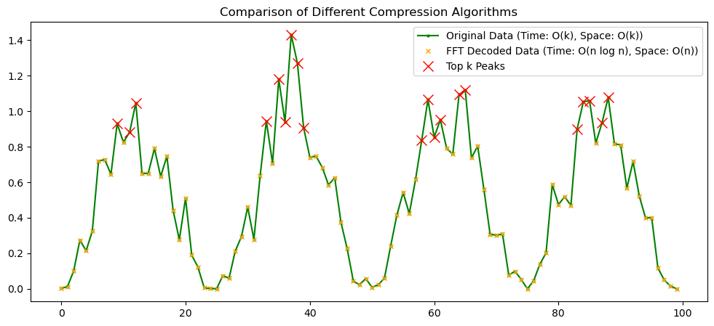
\includegraphics[width=0.9\linewidth, height=0.7\linewidth, keepaspectratio]{images/RPBC intro fig.png}
    \caption{Comparison of FFT and Naive Peak Selection Approaches}
    \label{fig:compression_algorithm}
\end{figure}

% Literature Review Section
\section{Literature Review}
The Fast Fourier Transform (FFT) is a widely used algorithm for encoding and decoding time series data due to its ability to efficiently transform signals into the frequency domain. Traditional FFT methods rely on a \textbf{divide-and-conquer strategy} to reduce the operation count to $\mathcal{O}(N \log N)$ when $N$ is factorizable~\cite{Gough2010FFT}. However, the computational and space overhead of FFT remains prohibitive for resource-constrained environments, such as real-time IoT systems~\cite{Thomas2021A}.

Recent optimizations in FFT, including parallel implementations, offer performance improvements but do not address fundamental memory limitations~\cite{Zhang2013Design}. To overcome these limitations, dynamic thresholding-based encoding algorithms have emerged as an alternative, reducing computational redundancy by selectively encoding key signal features~\cite{Cornforth2012Symbolic}. Similarly, divide-and-conquer methods have been applied in dynamic programming and encoding strategies to improve efficiency while maintaining signal characteristics~\cite{Itzhaky2016Deriving}.

These approaches demonstrate promising results for lightweight, high-accuracy data processing in time series communication, particularly in resource-limited IoT applications.
% Methodology Section
% \newpage
\section{Methodology}
This section provides a comprehensive description of the proposed recursive partitioning algorithm for \textbf{encoding} and \textbf{decoding} time series data.

\subsection{Encoding Process}
The \textbf{encoding process} compresses the time series by recursively partitioning it into segments and extracting key features using any of the statistical operations e.g max,mean,or ith-percentile etc which could be regarded as the base operation of our recursive method.
\newline
Given a time series \( X = \{x_1, x_2, \dots, x_N\} \), where \( N \) is the number of data points, the goal is to recursively partition \( X \) into smaller segments and store the \textbf{maximum value} in each segment if its length is below a predefined threshold \( k \).
\begin{itemize}
    \item \textbf{Base Case:} If \( |X| \leq k \), the encoded result is:
    \[
    E(X) = \max(X), \quad \text{where} \; X \; \text{is a segment of length} \; |X| \leq k.
    \]
    \item \textbf{Recursive Case:} If \( |X| > k \), the input is split into two halves:
    \[
    X_{\text{left}} = \{x_1, \dots, x_{\text{mid}}\}, \quad X_{\text{right}} = \{x_{\text{mid}+1}, \dots, x_N\},
    \]
    where \( \text{mid} = \left\lfloor \frac{N}{2} \right\rfloor \). The encoded result is:
    \[
    E(X) = E(X_{\text{left}}) \cup E(X_{\text{right}}).
    \]
\end{itemize}

% Pseudocode for Encoding Process
\begin{algorithm}[H] % Force exact placement using [H]
\caption{Encoding Algorithm}
\label{alg:encoding}
\begin{algorithmic}[1]
\STATE \textbf{Input:} Time series data $X$, Threshold $k$
\STATE \textbf{Output:} Encoded time series $E(X)$
\STATE
\IF{$\text{len}(X) \leq k$}
    \RETURN $\max(X)$ \hfill // Base case: return max value
\ENDIF
\STATE $\text{mid} \gets \text{floor}(\text{len}(X)/2)$
\STATE $\text{left\_part} \gets \text{Encode}(X[1:\text{mid}], k)$
\STATE $\text{right\_part} \gets \text{Encode}(X[\text{mid}+1:], k)$
\RETURN $\text{left\_part} + \text{right\_part}$ // concatenation of arrays
\end{algorithmic}
\end{algorithm}

The encoded representation consists of the maximum values extracted at each recursion level.

\subsection{Decoding Process}
The \textbf{decoding process} reconstructs the original time series using the encoded data.
\begin{itemize}
    \item \textbf{Base Case:} If the encoded sequence \( E(X) \) contains only one value \( v \), the reconstructed segment \( R(X) \) is:
    \[
    R(X) = \{v, v, \dots, v\}, \quad |R(X)| = N \; \text{(original segment length)}.
    \]
    \item \textbf{Recursive Case:} If \( |E(X)| > 1 \), the input is split into two halves, and each half is decoded recursively:
    \[
    R(X) = R(X_{\text{left}}) \cup R(X_{\text{right}}).
    \]
\end{itemize}
% Pseudocode for Decoding Process
Its pseudo-code is given below:
\begin{algorithm}[H] % Force exact placement using [H]
\caption{Decoding Algorithm}
\label{alg:decoding}
\begin{algorithmic}[1]
\STATE \textbf{Input:} Encoded data $E(X)$, Original length $N$, Threshold $k$
\STATE \textbf{Output:} Reconstructed time series $R(X)$
\STATE
\IF{$\text{len}(E(X)) == 1$}
    \RETURN $\{E(X)[1], E(X)[1], \dots, E(X)[1]\}$ of length $N$ \hfill // Base case
\ENDIF
\STATE $\text{half\_len} \gets \text{floor}(N/2)$
\STATE $\text{left\_part} \gets \text{Decode}(E(X)[1:\text{len}(E(X))/2], \text{half\_len}, k)$
\STATE $\text{right\_part} \gets \text{Decode}(E(X)[\text{len}(E(X))/2+1:], N - \text{half\_len}, k)$
\RETURN $\text{left\_part} + \text{right\_part}$
\end{algorithmic}
\end{algorithm}

Each segment is uniformly reconstructed using the maximum value stored in the encoded representation.

\subsection{Complexity Analysis}
The algorithm recursively divides the input \( X \) of size \( N \) into two halves until the segment size falls below a predefined threshold \( T \). Using the divide-and-conquer paradigm, the recurrence relation is:
\[
T(N) = 2T\left(\frac{N}{2}\right) + O(1).
\]
Applying the \textbf{Master Theorem}, we obtain:
\[
T(N) = O(N \log(N / k)).
\]
The space complexity is:
\[
O(N / k).
\]
All the steps above discussed are shown in fig \ref{fig:methodology} for fixed value of $k$ to help in understanding the mechanism of algorithm in detail.
\begin{figure}[!h]
    \centering
    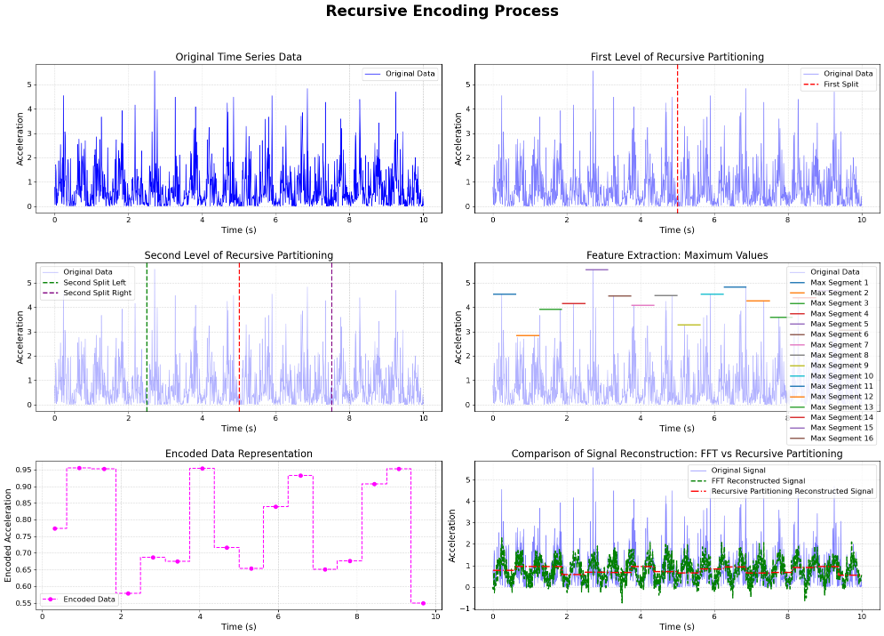
\includegraphics[width=0.9\linewidth, height=0.7\linewidth, keepaspectratio]{images/RPBC methodology.png}
    \caption{Visualization of stages of the application of RPBC}
    \label{fig:methodology}
\end{figure}
% Experiments Section
\section{Experiments}
The experiments were conducted on a system equipped with an AMD Ryzen 9 7950X 16-core Processor and 64GB RAM. The experiments utilized an open-source IoT accelerometer sensor time series dataset,Human Activity Recognition with Smartphones, representing real-world data generated by IoT devices in industrial applications ~\cite{Anguita2013APD}.

\subsection{Evaluation Metrics}
The performance of the proposed algorithm is evaluated using the following metrics:
\begin{enumerate}
    \item \textbf{Memory Usage (bytes):} Total size of the encoded arrays in bytes
    \item \textbf{Reconstruction Error (MSE):}
    \[
    \text{MSE} = \frac{1}{N} \sum_{i=1}^{N} (x_i - \hat{x}_i)^2,
    \]
    where \( x_i \) is the original time series value, and \( \hat{x}_i \) is the reconstructed value.
    \item \textbf{Execution Time:} Total time taken for encoding the array.
\end{enumerate}

\subsection{Experiments Overview}
We conducted three key experiments:
\begin{itemize}
    \item \textbf{Experiment 1: Hypothesis Testing on Small set of Uniformly Distributed Timeseries} - Evaluates the performance of the algorithm against different sizes of inputs, the impact of various thresholds, and its comparison with the FFT.
    \item \textbf{Experiment 2: Testing on the Real-world dataset} - Analyzes the effect of adaptive thresholds based on local signal variance and compares the proposed method with FFT-based compression techniques.
\end{itemize}
\begin{figure}[!h]
    \centering
    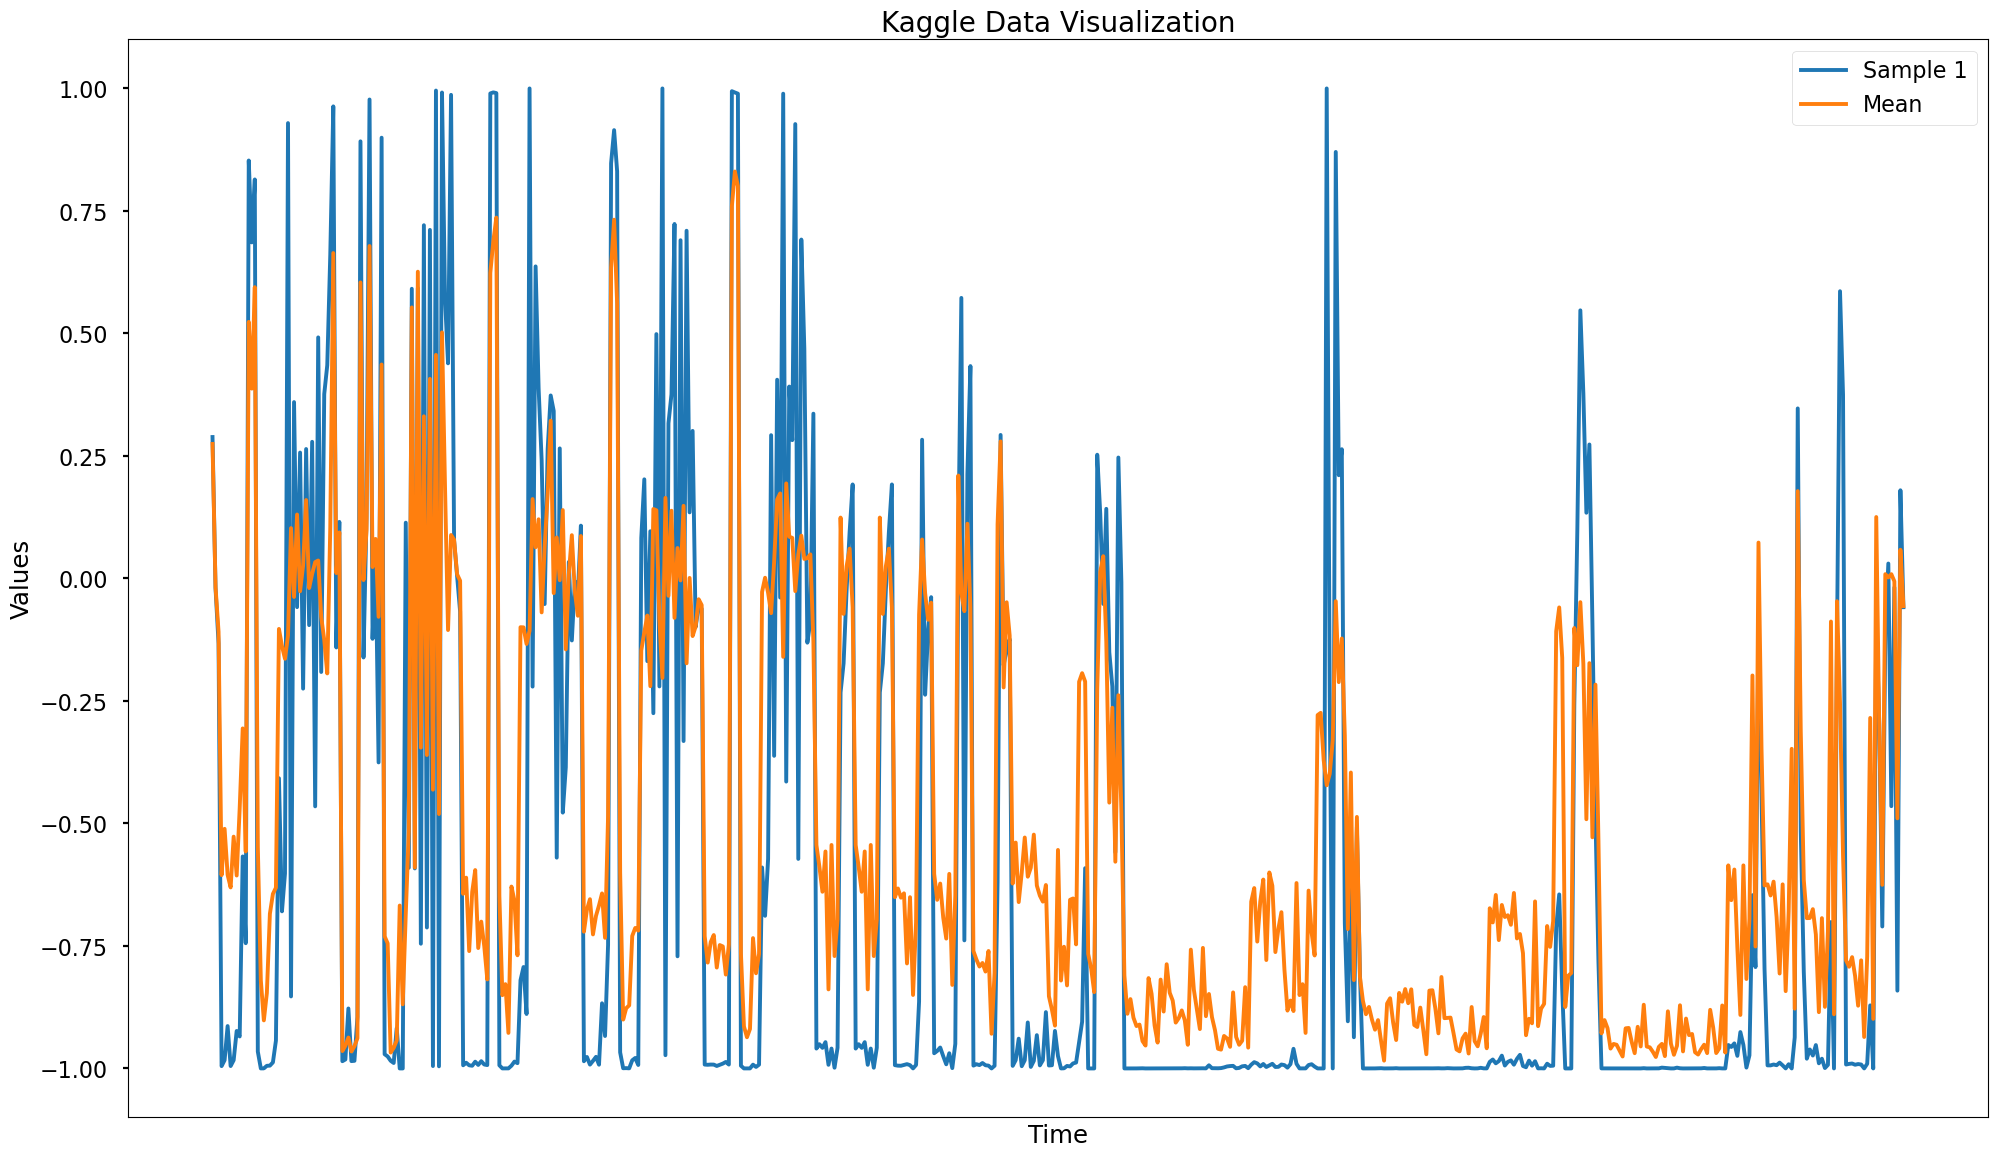
\includegraphics[width=0.7\linewidth, height=0.7\linewidth, keepaspectratio]{images/Experiment 2 Part a.png}
    \caption{Visualization of stages of the application of RPBC}
    \label{fig:A Sample Visualization of the Human Activity Recoginition Dataset }
\end{figure}
\subsection{Experiment Results}
\subsubsection{Comparative Analysis of RPBC with FFT on the Uniformly Distributed Time Series Dataset}
In this experiment, we applied the proposed algorithm to randomly distributed time series data of varying sizes and evaluated its performance against different threshold values $k$. Figure \ref{fig:1_part_a} illustrates that as the number of partitioned intervals decreases (i.e., larger thresholds), the reconstruction error increases. However, the results highlight a significant trade-off between runtime/memory usage and reconstruction accuracy.

For an optimal $k$, the mean squared error (MSE) becomes comparable to FFT-based reconstruction while consistently achieving better runtime and memory efficiency, as anticipated. For instance, in the given figure, 
$k = 184$ emerges as the most suitable parameter. This observation aligns with the well-known knee-point problem (or L-method), which is commonly used in techniques like k-means clustering to determine the optimal number of clusters by balancing performance trade-offs \cite{JSSv061i06}. 
\begin{figure}[!h]
    \centering
    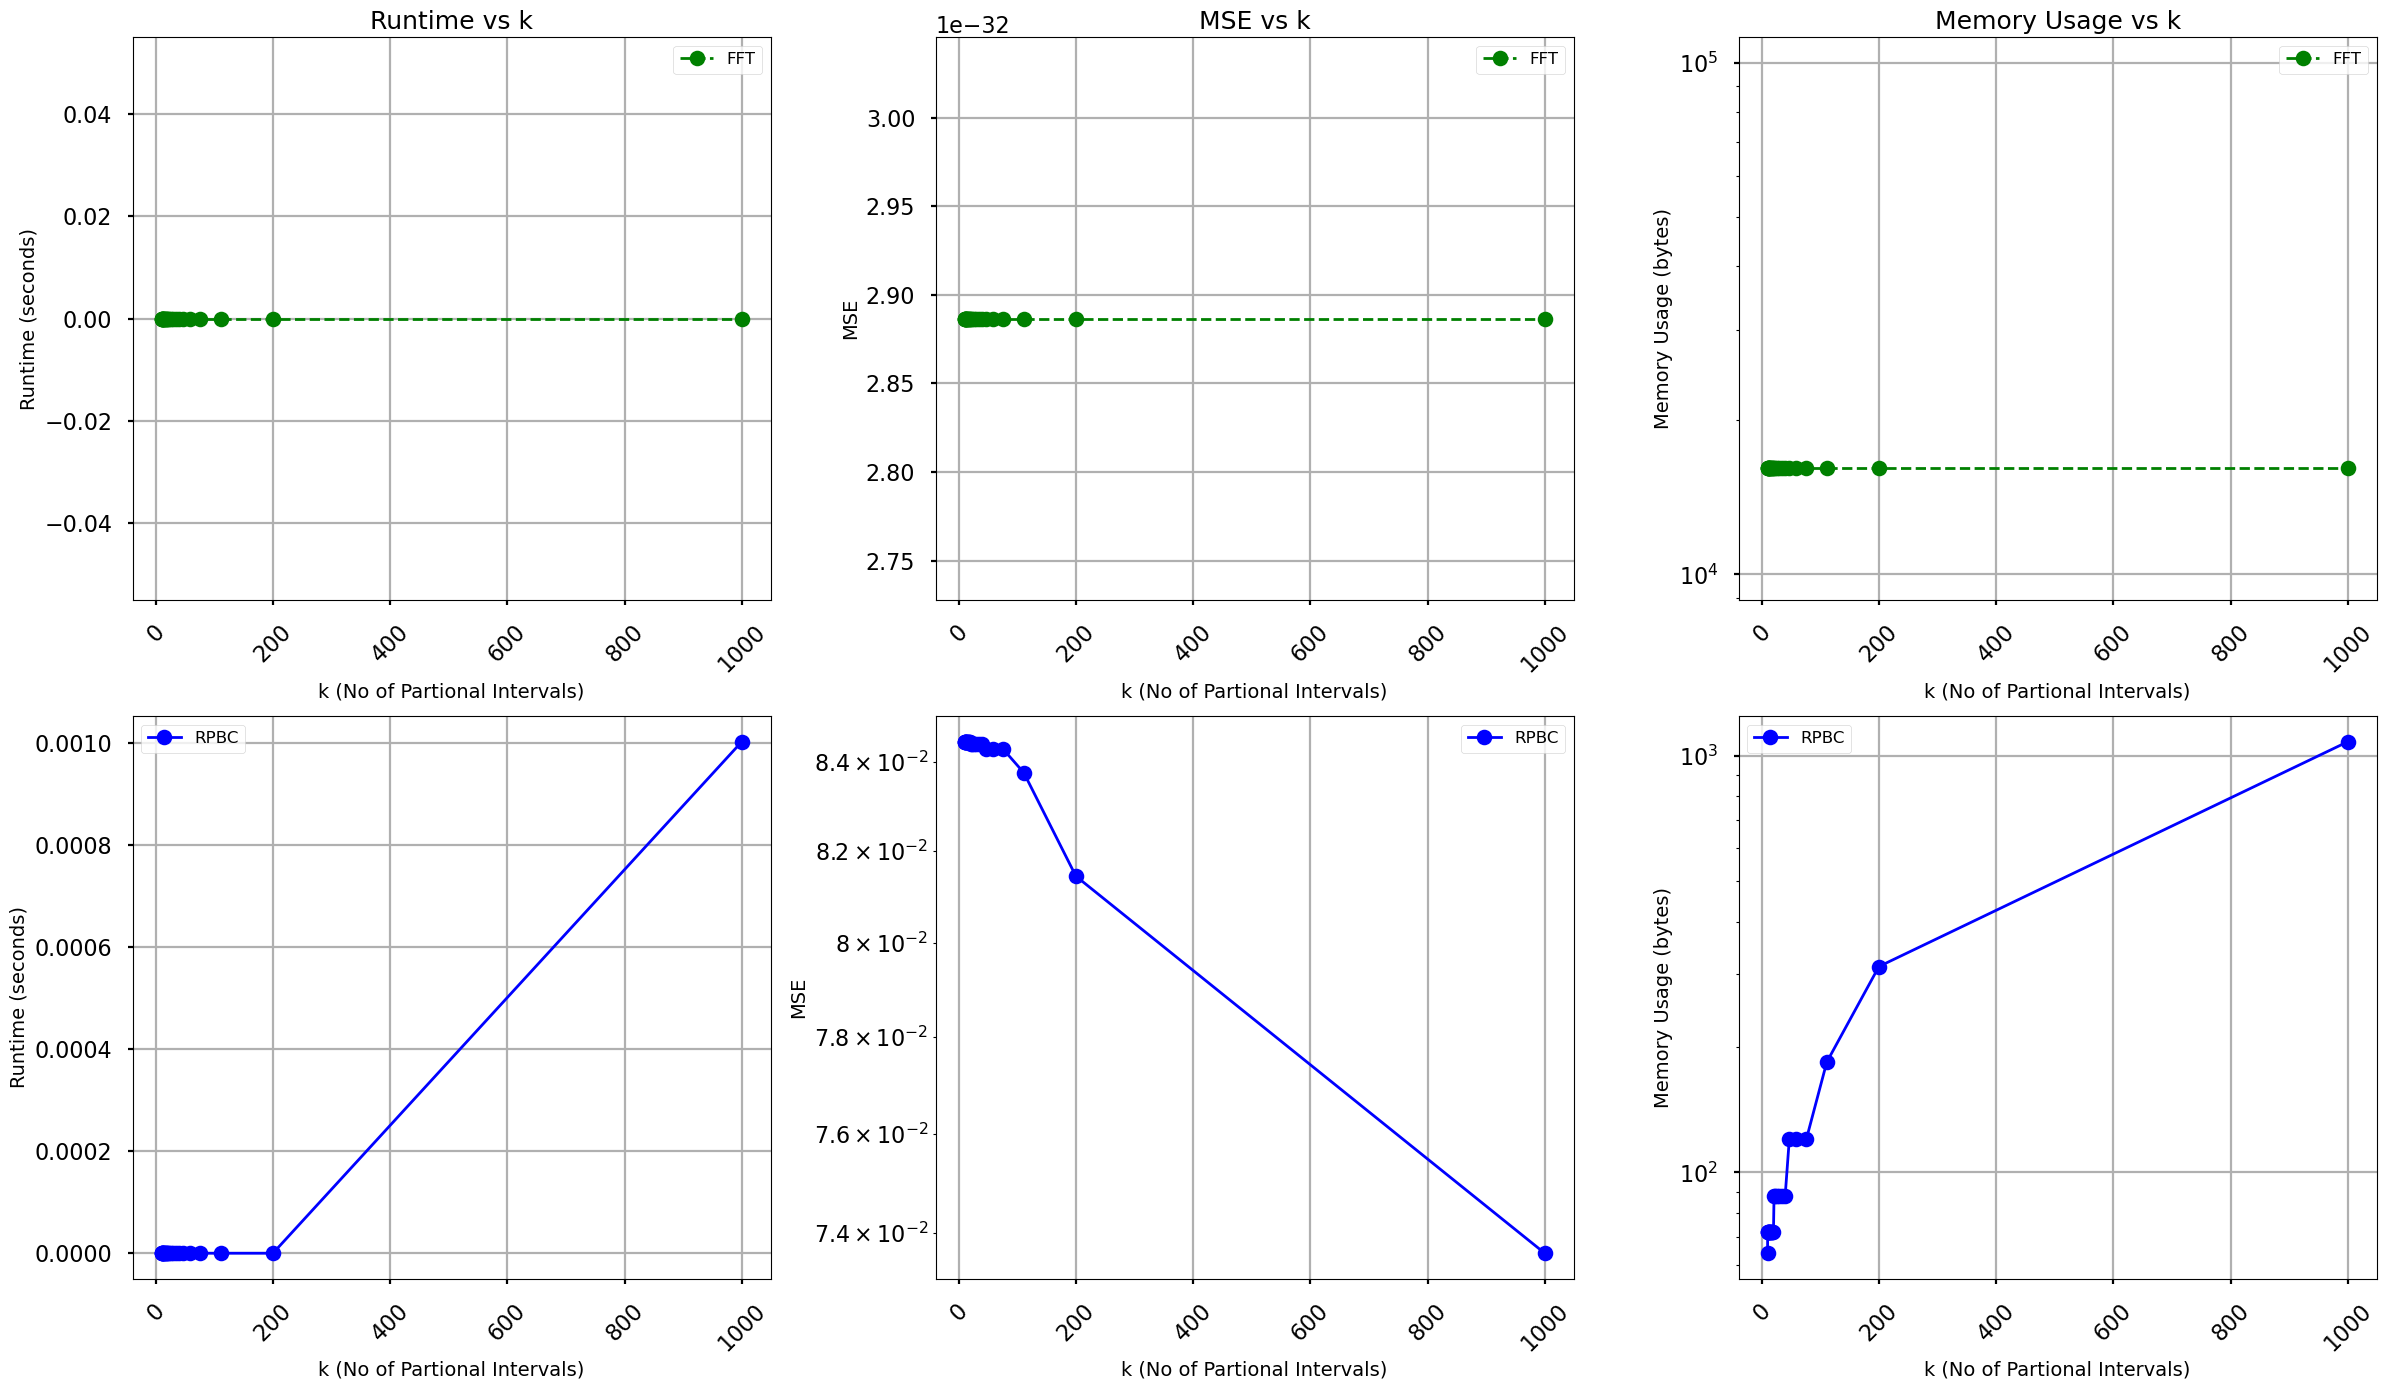
\includegraphics[width=1\linewidth, height=1\linewidth,keepaspectratio]{images/Experiment 1 Part a.png}
    \caption{Comparison of FFT and RPBC against different thresholds for fixed size of input i.e $10^3$}
    \label{fig:1_part_a}
\end{figure}

\begin{figure}[!h]
    \centering
    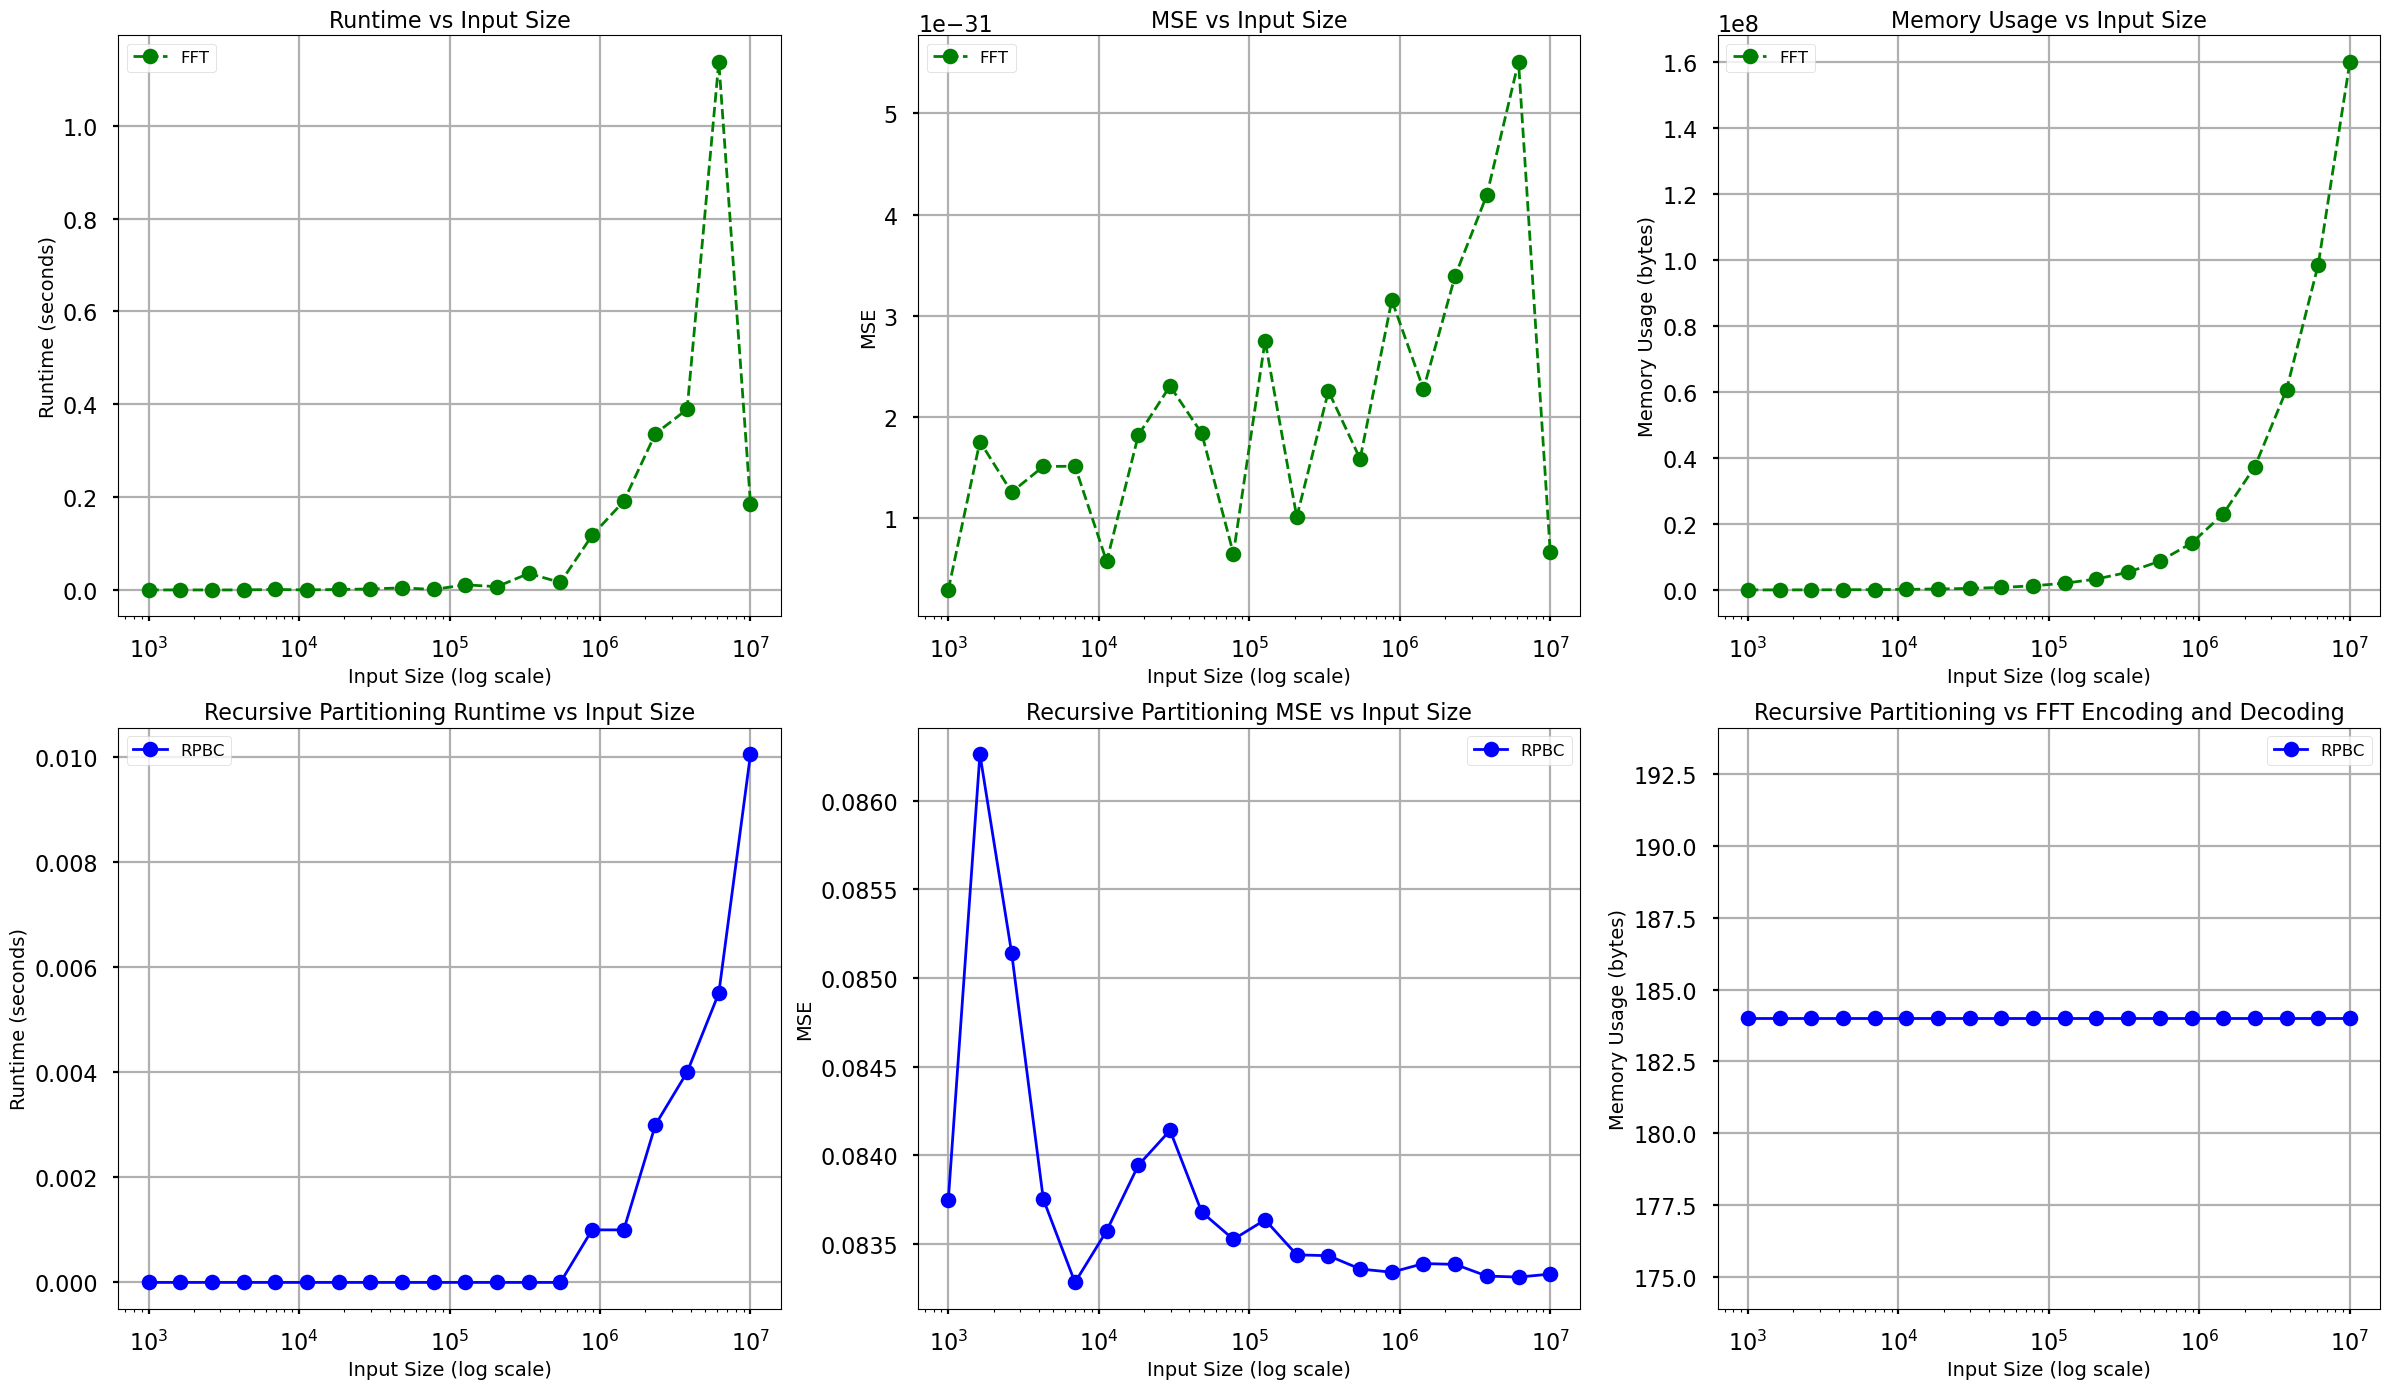
\includegraphics[width=1\linewidth, height=1\linewidth,keepaspectratio]{images/Experiment 1 Part b.png}
    \caption{Comparison of FFT and RPBC against different input size of data}
    \label{fig:1_part_b}
\end{figure}
To further validate the asymptotic behavior of our encoding algorithm, we compared its performance against FFT by fixing $k$ and varying the input sizes to observe the Big-O curves. Figure \ref{fig:1_part_b} shows that the runtime curve for the Recursive Partition-Based Compression (RPBC) algorithm follows the expected $O (NlogN)$ behavior. However, the runtime scale is consistently reduced compared to FFT, demonstrating the efficiency of our approach. For memory usage, our algorithm successfully reconstructs the signal using only 184 points, while FFT's memory requirements grow logarithmically and are "off the charts" for larger input sizes. Nevertheless, limitations exist in the reconstruction accuracy: the minimum achievable error for RPBC is approximately 0.08, whereas FFT reconstructs the signal with near-perfect accuracy due to the absence of resource constraints
\subsubsection{Comparative Analysis of RPBC with FFT on the Opensource Dataset}
We tested the performance of the proposed Recursive Partition-Based Compression (RPBC) algorithm on the Human Activity Recognition Dataset \cite{Anguita2013APD} to compare it with the Fast Fourier Transform (FFT).

Figure \ref{fig:2b} shows that RPBC clearly outperforms FFT in terms of runtime and memory usage, while FFT achieves better reconstruction accuracy. At $k=20$, RPBC achieves a comparable reconstruction error to FFT but with significant gains in efficiency. The term 'comparable reconstruction' depends on the application: in resource-constrained scenarios like IoT or wearable devices, RPBC’s small error is often acceptable given its reduced computational cost. Figure \ref{fig:2c} further demonstrates that lower values of $k$ allow RPBC to reconstruct the signal efficiently using only a limited number of key points, achieving a compression ratio of over $50$ \%. This balance between accuracy and compression makes RPBC highly suitable for applications requiring both speed and memory efficiency. In summary, while FFT ensures high reconstruction accuracy, RPBC provides a practical trade-off by optimizing runtime, memory usage, and compression ratio, making it ideal for resource-limited applications.


\begin{figure}[!h]
    \centering
    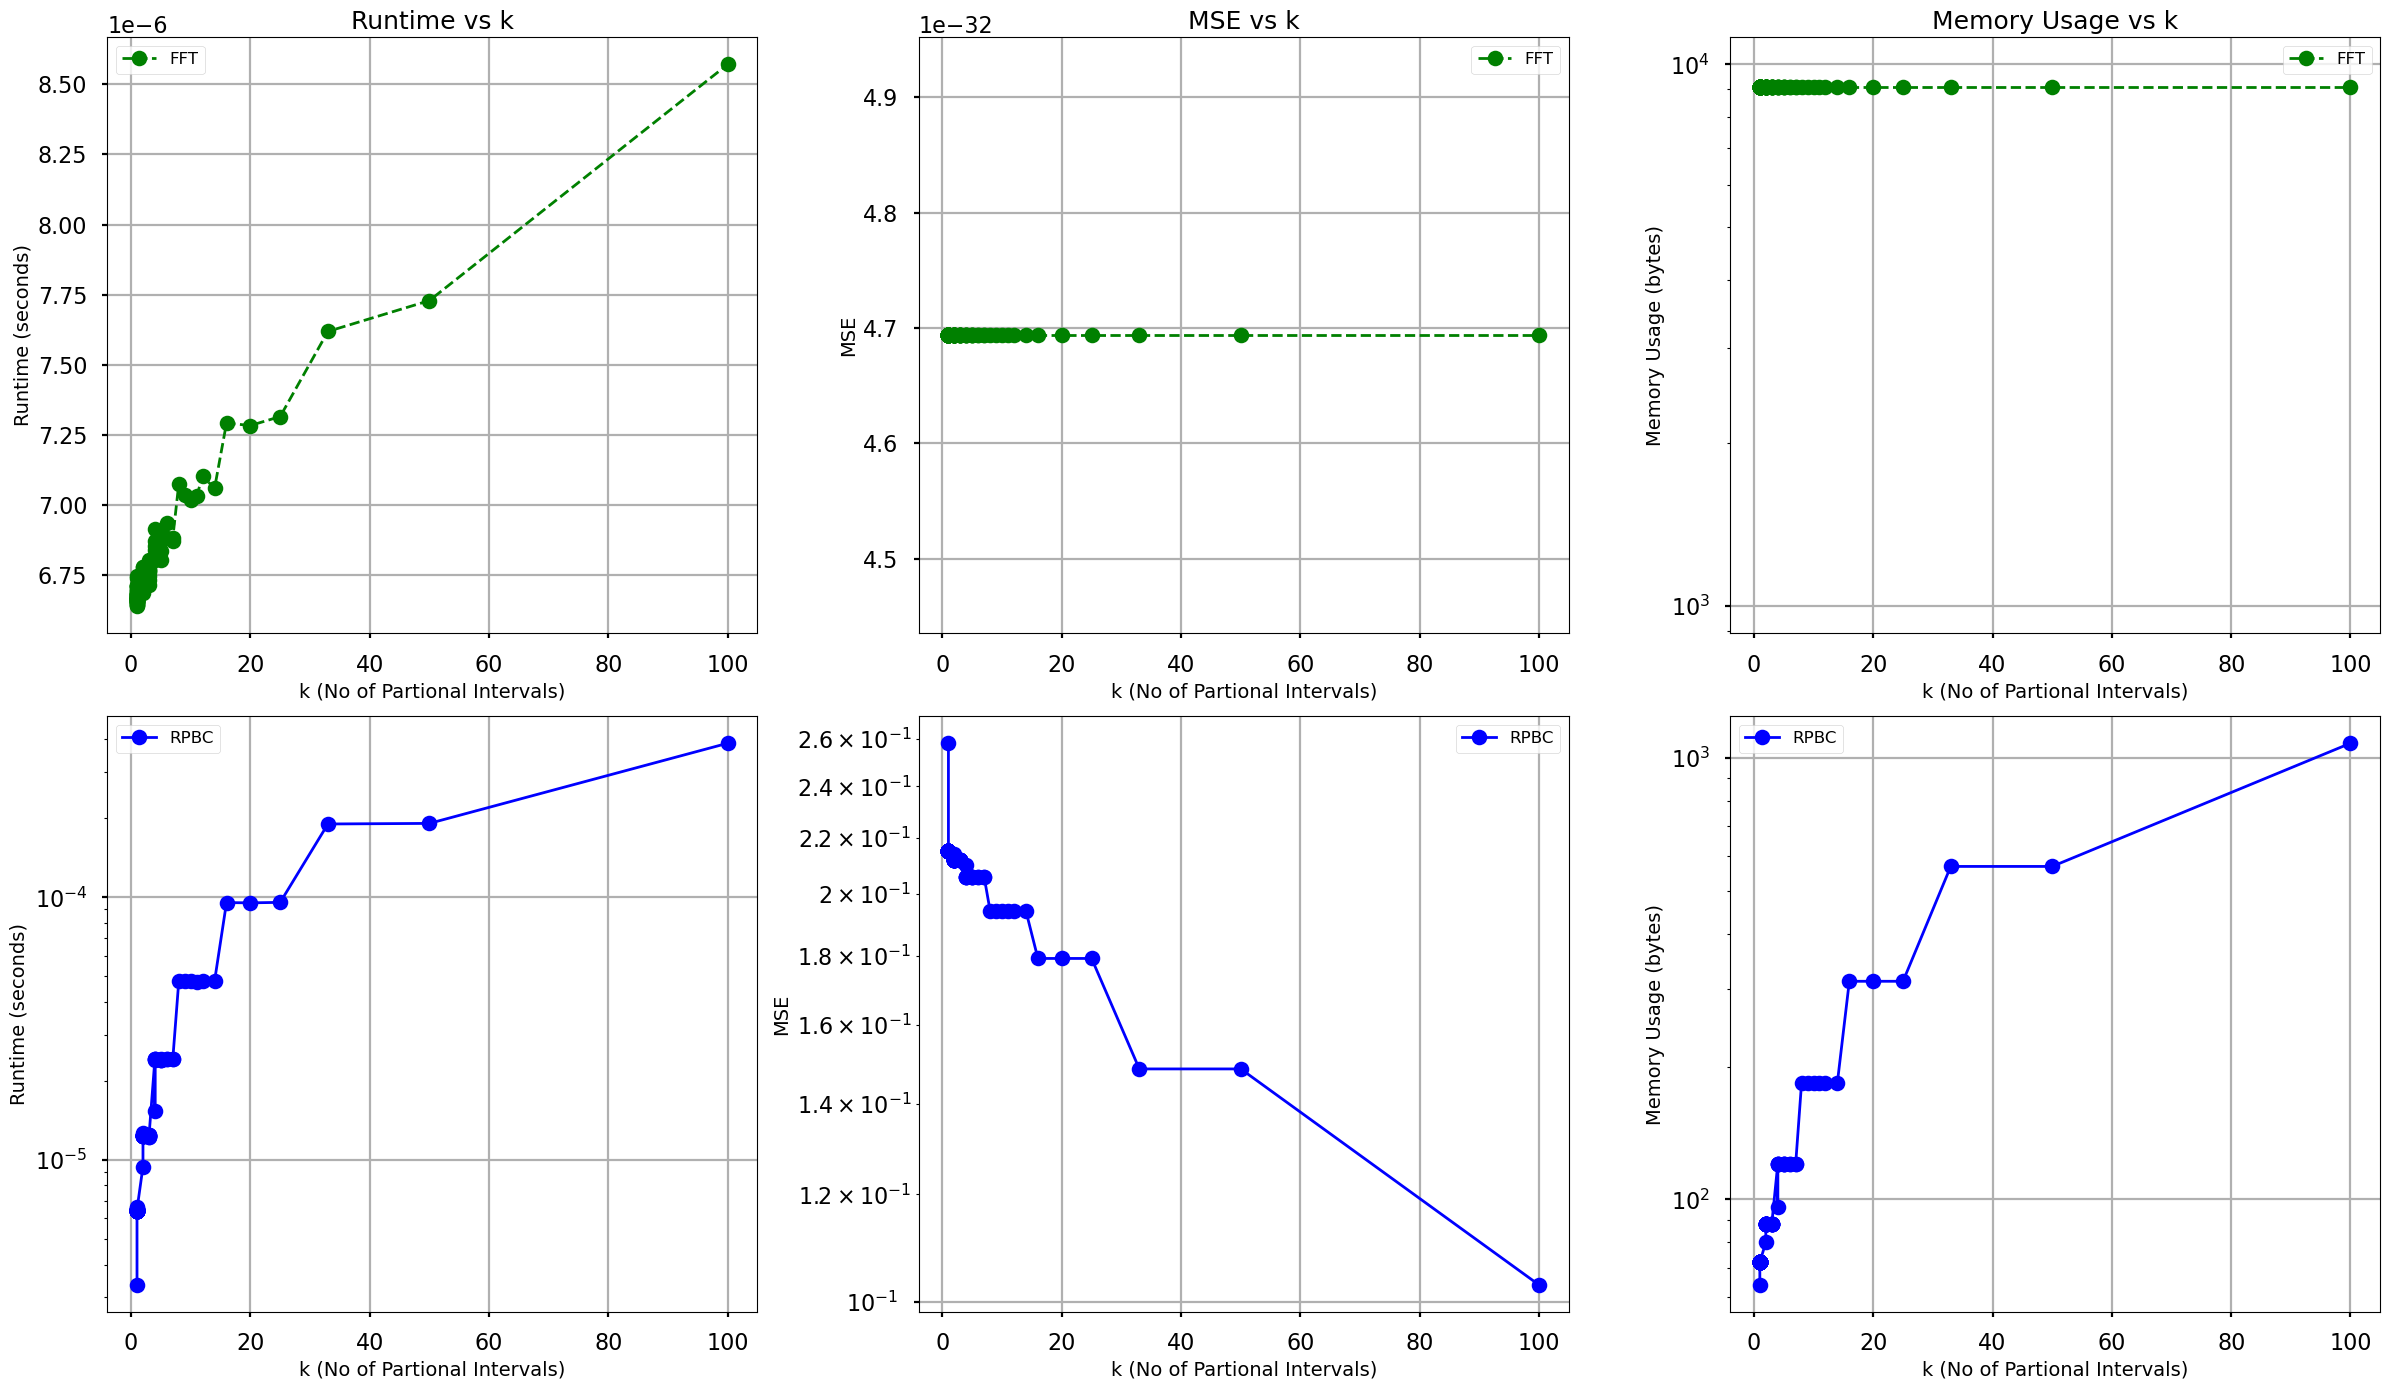
\includegraphics[width=0.9\linewidth, height=0.7\linewidth, keepaspectratio]{images/Experiment 2 Part b.png}
    \caption{Comparison of FFT with RPBC on Human Activity Recoginition Dataset}
    \label{fig:2b}
\end{figure}
\begin{figure}[!h]
    \centering
    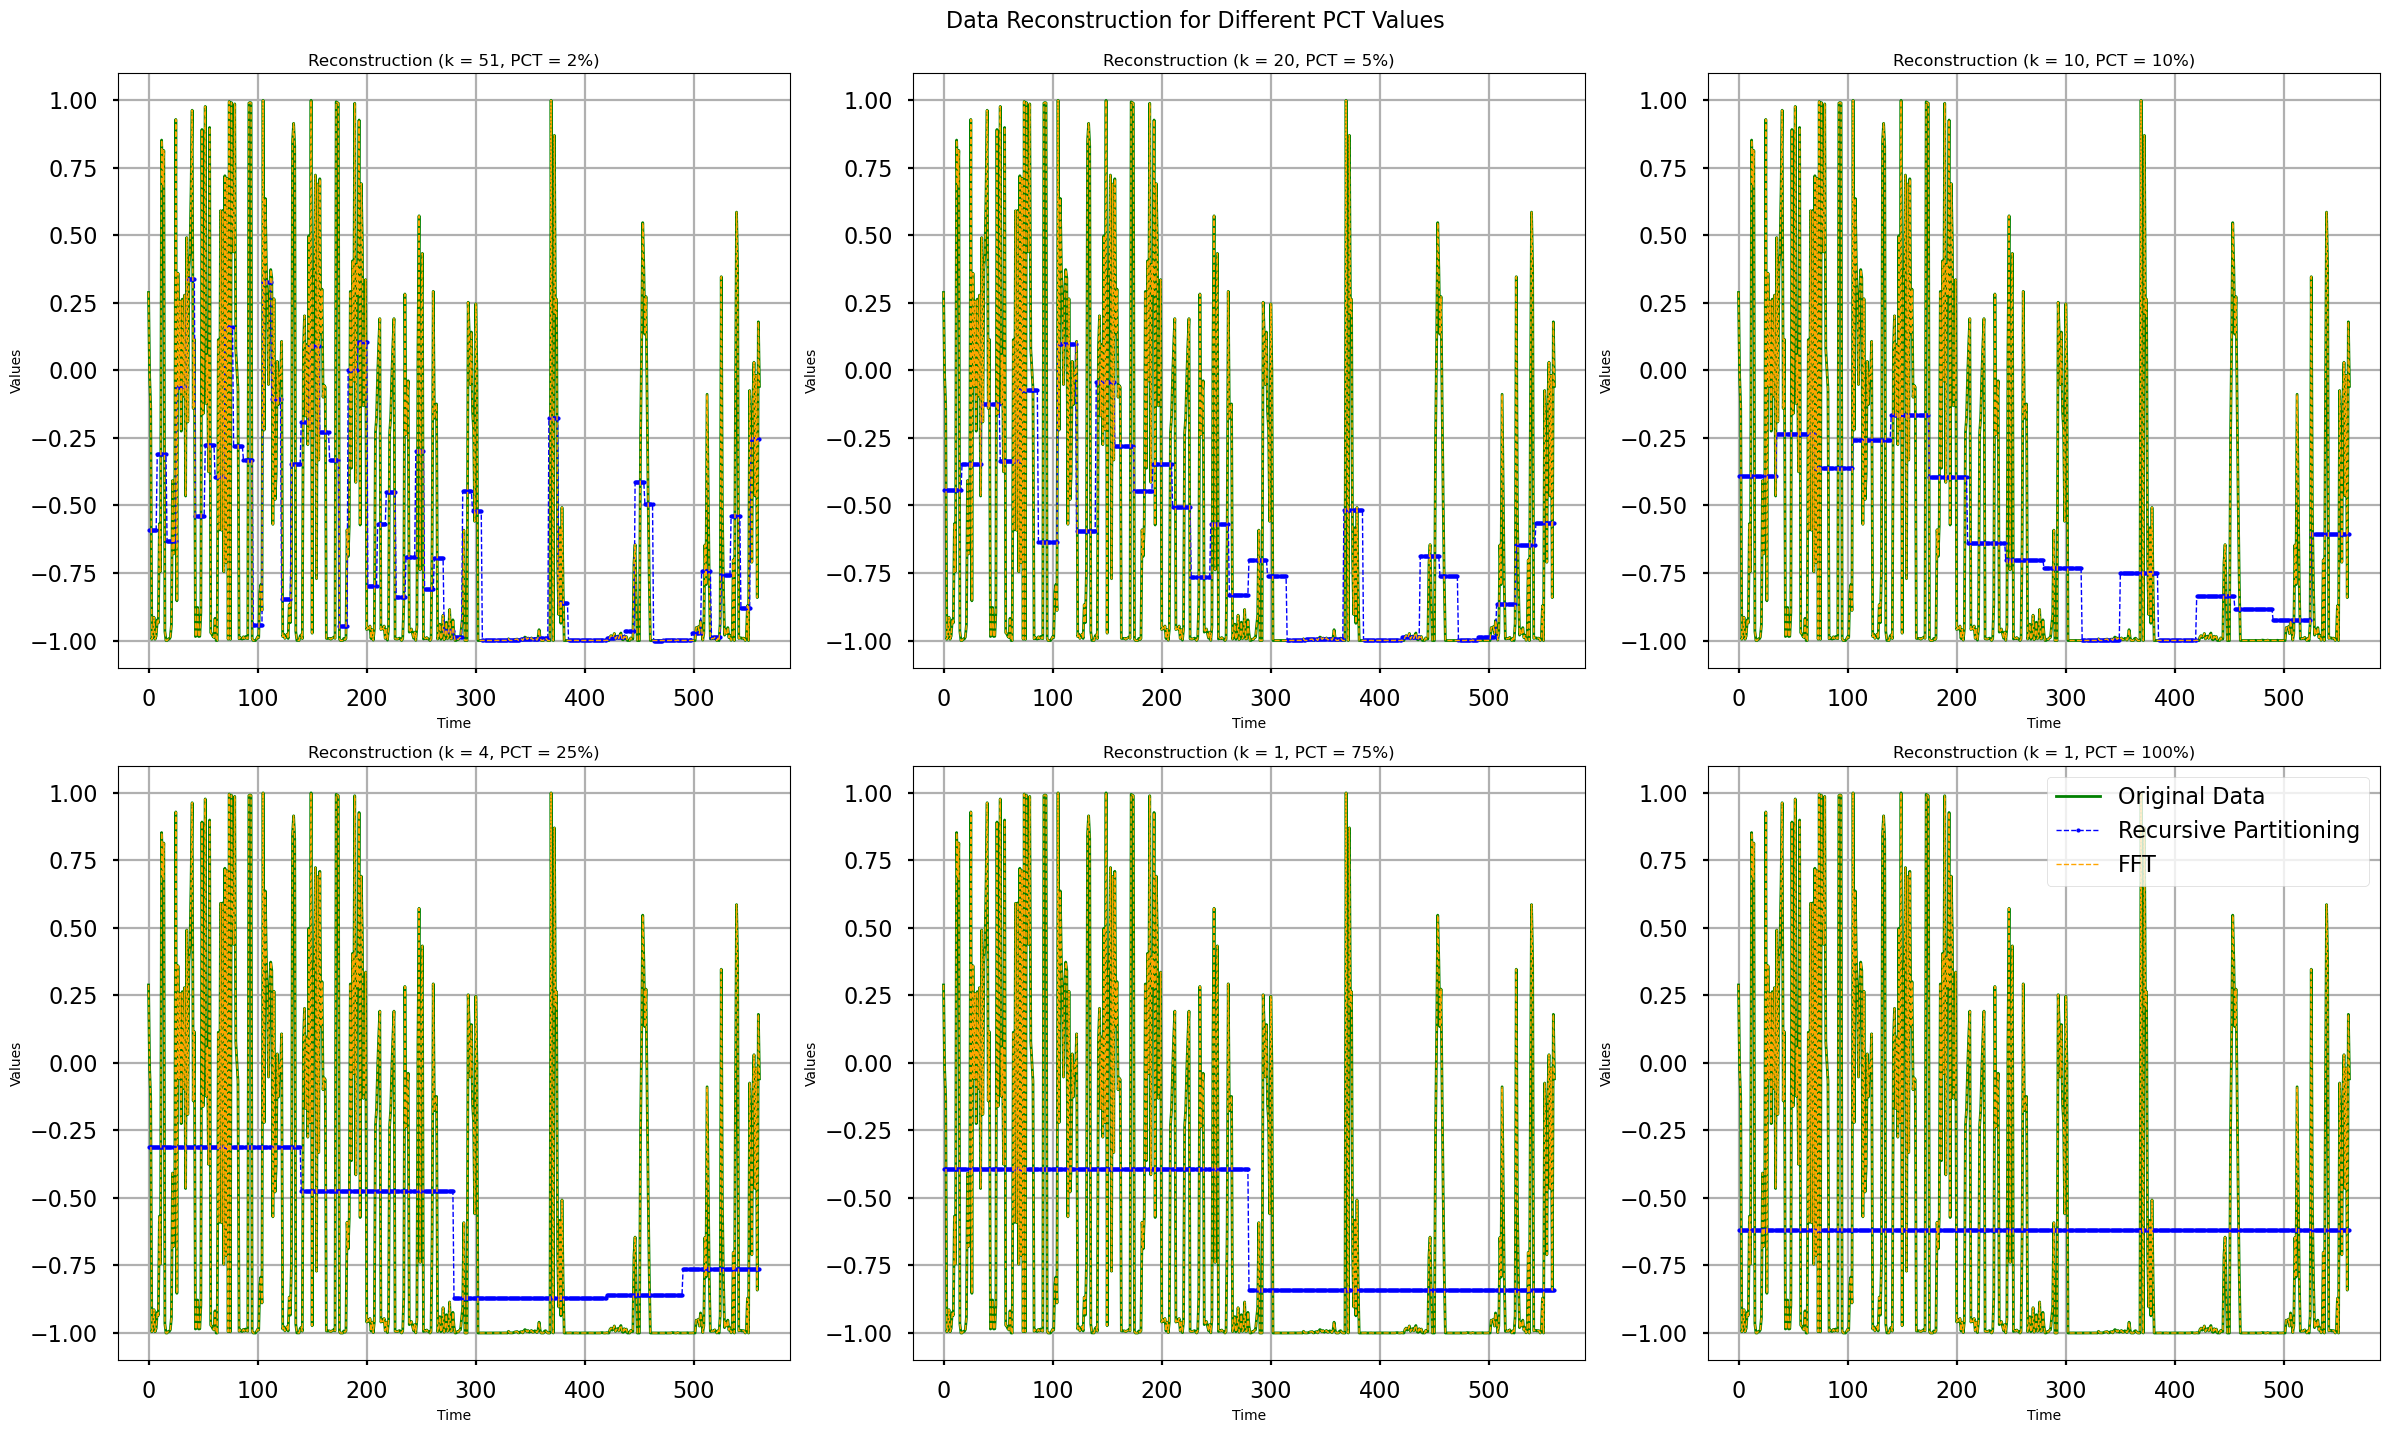
\includegraphics[width=0.9\linewidth, height=0.7\linewidth, keepaspectratio]{images/Experiment 2 Part c.png}
    \caption{Visualization of Reconstructed Signals from FFT \& RPBC}
    \label{fig:2c}
\end{figure}

\section{Discussion}

\subsection{Selection Strategy of Parameter $k$}
The \textbf{knee-value} plays a critical role in balancing compression efficiency and reconstruction accuracy. As observed in the experiments, selecting an optimal threshold \( k \) ensures a trade-off where the algorithm achieves significant compression while maintaining a reasonable reconstruction error. 

Figures \ref{fig:2b} and \ref{fig:2c} illustrate that values like \( k = 20 \) or \( k = 180 \) act as knee points, achieving near-optimal performance because the static thresholds may not generalize well for signals with varying complexity.

\subsection{Variant of RPBC in case of high-temporal variation in the Data: Intermittent Time Series Datasets}
The current algorithm uses a single threshold \( k \) for partitioning. This can be further improved by introducing \textbf{dual thresholds} \( k_1 \) and \( k_2 \):
\begin{itemize}
    \item \( k_1 \): Used for identifying critical regions of high variability in the signal (e.g., peaks or anomalies).
    \item \( k_2 \): Used for flatter, low-variability regions where higher compression is acceptable.
\end{itemize}
By dynamically adjusting $k1$ \& $k2$ based on signal variance or entropy, the algorithm can achieve a more efficient balance between compression and reconstruction accuracy. This approach is particularly effective for signals with mixed complexity, such as those observed in industrial sensor data. The inspiration for this improvement comes from Molding Manufacturing Systems (MMS), where accelerometer or pressure signals often exhibit a tidal-like behavior: one portion of the signal has a high concentration of meaningful data, while the other half is dominated by zeros or low-activity regions \cite{s22166165}. In such cases, employing FFT can be computationally expensive, as it processes the entire signal uniformly. Similarly, the initial version of RPBC may redundantly encode unnecessary information, leading to inefficiencies. To address this, dynamically adjusting $k1$ \& $k2$ allows the algorithm to allocate smaller thresholds for high-variance regions (preserving more detail) and larger thresholds for low-variance or sparse regions (maximizing compression). This targeted approach ensures that critical features are retained while avoiding the overhead of encoding irrelevant data. The resulting recursive form of the algorithm is as follows:

Given a time series \( X = \{x_1, x_2, \dots, x_N\} \), where \( N \) is the number of data points, the goal is to recursively partition \( X \) and apply different thresholds \( k_1 \) and \( k_2 \) to the left and right segments based on the \textbf{concentration of non-zero values}.


\noindent \textbf{1. Base Case:} If the segment length \( |X| \leq k \) (where \( k \) is the minimum threshold for stopping), extract the \textbf{maximum value} of the segment \( X \):
\[
E(X) = \max(X).
\]

\noindent \textbf{2. Recursive Case:} Split the segment \( X \) into two parts:
\[
X_{\text{left}} = \{x_1, x_2, \dots, x_{\text{mid}}\}, \quad X_{\text{right}} = \{x_{\text{mid}+1}, \dots, x_N\},
\]
where \( \text{mid} = \left\lfloor \frac{N}{2} \right\rfloor \).

For each segment, dynamically adjust the thresholds \( k_{\text{left}} \) and \( k_{\text{right}} \) based on the \textbf{concentration of non-zeros} \( c(X) \):
\[
k_{\text{left}} = f(c(X_{\text{left}})), \quad k_{\text{right}} = f(c(X_{\text{right}})).
\]
Here, \( f \) is a function that maps the concentration of non-zeros to a threshold value. The function \( f \) can be defined as:
\[
f(c) = \begin{cases} 
k_{\text{min}}, & \text{if } c(X) > \tau, \\
k_{\text{max}}, & \text{otherwise}.
\end{cases}
\]
where \( \tau \) is a predefined threshold for high concentration.

The recursive encoding function can then be expressed as:
\[
E(X) = 
\begin{cases} 
\max(X), & \text{if } |X| \leq k, \\
E(X_{\text{left}}, k_{\text{left}}) \cup E(X_{\text{right}}, k_{\text{right}}), & \text{otherwise}.
\end{cases}
\]

The pseudocode for encoding with dynamic thresholds \( k_1 \) and \( k_2 \) is as follows:

\begin{algorithm}[H]
\caption{Recursive Encoding with Dynamic Thresholds}
\label{alg:dynamic_encoding}
\begin{algorithmic}[1]
\STATE \textbf{Input:} Time series data \( X \), thresholds \( k_{\text{min}}, k_{\text{max}} \)
\STATE \textbf{Output:} Encoded time series \( E(X) \)
\STATE
\IF{\text{len}(X) \( \leq k_{\text{min}} \)}
    \RETURN \( [\max(X)] \) \COMMENT{Base case: Extract key feature}
\ENDIF
\STATE Split \( X \) into two parts:
\STATE \hspace{0.5cm} \( X_{\text{left}} \gets X[1:\text{mid}] \), \( X_{\text{right}} \gets X[\text{mid}+1:N] \)
\STATE Compute the concentration of non-zeros:
\STATE \hspace{0.5cm} \( c_{\text{left}} \gets \frac{\text{count\_nonzeros}(X_{\text{left}})}{\text{len}(X_{\text{left}})} \)
\STATE \hspace{0.5cm} \( c_{\text{right}} \gets \frac{\text{count\_nonzeros}(X_{\text{right}})}{\text{len}(X_{\text{right}})} \)
\STATE Adjust thresholds dynamically:
\STATE \hspace{0.5cm} \( k_{\text{left}} \gets \text{adjust\_threshold}(c_{\text{left}}, k_{\text{min}}, k_{\text{max}}) \)
\STATE \hspace{0.5cm} \( k_{\text{right}} \gets \text{adjust\_threshold}(c_{\text{right}}, k_{\text{min}}, k_{\text{max}}) \)
\STATE Recursively encode the left and right parts:
\STATE \hspace{0.5cm} \( E_{\text{left}} \gets \text{EncodeWithDynamicK}(X_{\text{left}}, k_{\text{left}}, k_{\text{max}}) \)
\STATE \hspace{0.5cm} \( E_{\text{right}} \gets \text{EncodeWithDynamicK}(X_{\text{right}}, k_{\text{min}}, k_{\text{right}}) \)
\STATE \RETURN \( E_{\text{left}} \cup E_{\text{right}} \) \COMMENT{Combine results}
\end{algorithmic}
\end{algorithm}

\begin{itemize}
    \item \textbf{Concentration of Non-Zeros:}  
    The concentration \( c(X) \) for a segment \( X \) is defined as:
    \[
    c(X) = \frac{\text{Number of non-zero values in } X}{|X|}.
    \]

    \item \textbf{Threshold Adjustment:}  
    The thresholds \( k_{\text{left}} \) and \( k_{\text{right}} \) are adjusted dynamically using the function \( f \), which maps the concentration of non-zeros to a threshold:
    \[
    k = f(c) = 
    \begin{cases} 
    k_{\text{min}}, & \text{if } c(X) > \tau, \\
    k_{\text{max}}, & \text{otherwise}.
    \end{cases}
    \]
    Here, \( \tau \) is a predefined threshold that determines the concentration level for high detail.

    \item \textbf{Dynamic Partitioning:}  
    The recursion continues with adjusted thresholds \( k_{\text{left}} \) and \( k_{\text{right}} \) until the segment size becomes smaller than \( k_{\text{min}} \), at which point the base case is triggered.
\end{itemize}

\subsubsection{Application in Pattern Recognition and Machine Learning}
Once can also use the Machine Learning algorithms by carefully crafting the optimizing function to find the best approximation in the partional space such as 
\[
y(t) = a \cdot x(t) + b \cdot x(t) + c \cdot x(t),
\]
where \( x(t) \) represent partition of the input signal. Using machine learning techniques, coefficients \( a \), \( b \), and \( c \) can be estimated during the \textbf{pre-production stage} to fit the variance in the data. 

\subsection{Limitations}
Despite its advantages, the RPBC algorithm has some limitations:
\begin{enumerate}
    \item \textbf{Reconstruction Accuracy}: The algorithm introduces a minimum error (e.g., ~0.08) that cannot match FFT’s near-perfect reconstruction. This makes it less suitable for applications requiring high precision.
    \item \textbf{Static Thresholding}: The use of a fixed threshold \( k \) may not generalize well for all signals. Dynamic thresholding strategies, such as \( k_1 \) and \( k_2 \), need further exploration.
    \item \textbf{Loss of Fine-Grained Details}: In regions with high-frequency variations, the algorithm may fail to preserve finer details, leading to inaccuracies in applications requiring frequency-domain analysis.
    \item \textbf{Limited Non-Uniform Reconstruction}: The current method uses uniform expansion for decoding, which may introduce artifacts. Incorporating \textbf{non-uniform reconstruction} techniques, such as linear interpolation or spline methods, could improve accuracy.
\end{enumerate}


\section{Conclusion}
This research presents a recursive partitioning algorithm (RPBC) for efficiently encoding and decoding IoT time series data. The method achieves over 50 \% compression while maintaining acceptable reconstruction accuracy, outperforming FFT in runtime and memory usage for resource-constrained systems.
Experiments on synthetic and real-world datasets demonstrate RPBC’s ability to balance compression efficiency and reconstruction fidelity, with dynamic thresholds enhancing its adaptability for signals with varying complexity. Future work will focus on improving reconstruction accuracy using non-uniform decoding and automating adaptive threshold selection for broader real-time applications. RPBC offers a practical and scalable solution for IoT systems requiring lightweight data compression.
% References
\bibliographystyle{IEEEtran}
\bibliography{mybib}
\newpage
\appendix
\section{Implementation Code}

This appendix provides the Python implementation for the recursive encoding and decoding functions, FFT-based encoding and decoding, and the experimental setup for performance comparison. For more details, please visit the Github Repo . \href{https://github.com/ghafoorharis/cs5850-algorithms/tree/main/project}{https://github.com/ghafoorharis/cs5850-algorithms}

\begin{verbatim}
import numpy as np
import sys
import time
import timeit
from scipy.fftpack import fft, ifft
import pandas as pd

# Recursive Encoding Function
def encode(data, threshold):
    """
    Recursively encodes the input data by partitioning it into segments
    and taking the mean value for each segment if its length <= threshold.

    Parameters:
    - data: Input time series (list or numpy array)
    - threshold: Minimum segment size for stopping recursion

    Returns:
    - Encoded data (list of means)
    """
    if len(data) <= threshold:
        return [np.mean(data)]  # Base case: compute mean of the segment
    mid = len(data) // 2  # Split data into two halves
    return encode(data[:mid], threshold) + encode(data[mid:], threshold)

# Recursive Decoding Function
def decode(encoded_data, original_length, threshold):
    """
    Decodes the recursively encoded data by reconstructing the original length.

    Parameters:
    - encoded_data: Encoded list of means
    - original_length: Length of the original time series
    - threshold: Minimum segment size used for encoding

    Returns:
    - Reconstructed data (list)
    """
    if len(encoded_data) == 1:
        return [encoded_data[0]] * original_length  # Base case: expand segment
    half_len = original_length // 2
    # Recursively reconstruct left and right halves
    left = decode(encoded_data[:len(encoded_data)//2], half_len, threshold)
    right = decode(encoded_data[len(encoded_data)//2:], original_length - half_len, threshold)
    return left + right
\end{verbatim}

\subsection{Error Calculation and FFT Functions}
The following functions compute the Mean Squared Error (MSE) between original and reconstructed signals and implement FFT-based encoding and decoding.

\begin{verbatim}
# Mean Squared Error Function
def mse(original, reconstructed):
    """
    Computes the Mean Squared Error between the original and reconstructed signals.

    Parameters:
    - original: Original time series (list or numpy array)
    - reconstructed: Reconstructed time series (list or numpy array)

    Returns:
    - MSE value (float)
    """
    return np.mean((np.array(original) - np.array(reconstructed)) ** 2)

# FFT-Based Encoding Function
def fft_encode(data):
    """
    Performs FFT encoding on the input data.

    Parameters:
    - data: Input time series (list or numpy array)

    Returns:
    - FFT transformed data (numpy array)
    """
    return fft(data)

# FFT-Based Decoding Function
def fft_decode(encoded_data):
    """
    Decodes FFT-encoded data using Inverse FFT.

    Parameters:
    - encoded_data: FFT-encoded data (numpy array)

    Returns:
    - Reconstructed signal (real values)
    """
    return ifft(encoded_data).real
\end{verbatim}

\subsection{Memory Usage and Runtime Measurement}
The following helper functions calculate memory usage and runtime performance.

\begin{verbatim}
# Memory Usage Calculation
def memory_usage(data):
    """
    Computes the memory usage of the input data in bytes.

    Parameters:
    - data: Input data (list or numpy array)

    Returns:
    - Memory size in bytes (int)
    """
    return sys.getsizeof(data)

# Precise Runtime Measurement
def measure_runtime(func, *args):
    """
    Measures the runtime of a function using timeit.

    Parameters:
    - func: Function to measure
    - *args: Arguments for the function

    Returns:
    - Runtime in seconds (float)
    """
    runtime = timeit.timeit(lambda: func(*args), number=1)
    return runtime
\end{verbatim}

\subsection{Experimental Setup: Random Time Series with FFT Comparison}
The following function tests the recursive algorithm and FFT on random time series data of varying sizes and calculates runtime, memory usage, and reconstruction errors.

\begin{verbatim}
# Random Time Series Test with FFT Comparison
def random_time_series_experiment_with_fft(sizes, PCT):
    """
    Runs experiments to compare recursive encoding/decoding with FFT-based methods.

    Parameters:
    - sizes: List of time series sizes to test
    - PCT: Percentage threshold for recursive partitioning

    Returns:
    - DataFrame containing results for runtime, MSE, and memory usage
    """
    # Initialize result containers
    runtimes_recursive = []
    runtimes_fft = []
    errors_recursive = []
    errors_fft = []
    memory_fft = []
    memory_recursive = []

    for size in sizes:
        np.random.seed(0)  # Set random seed for reproducibility
        data = np.random.random(int(size))  # Generate random time series
        threshold = int(data.shape[0] * PCT / 100)  # Threshold based on percentage

        # Recursive Partitioning Encoding/Decoding
        start = time.time()
        encoded_recursive = encode(data, threshold)
        end = time.time()
        reconstructed_recursive = decode(encoded_recursive, len(data), threshold)
        runtimes_recursive.append(end - start)
        errors_recursive.append(mse(data, reconstructed_recursive))

        # FFT Encoding/Decoding
        start = time.time()
        encoded_fft = fft_encode(data)
        end = time.time()
        reconstructed_fft = fft_decode(encoded_fft)
        runtimes_fft.append(end - start)
        errors_fft.append(mse(data, reconstructed_fft))

        # Memory Usage
        memory_fft.append(memory_usage(encoded_fft))
        memory_recursive.append(memory_usage(encoded_recursive))

    # Compile results into a DataFrame
    dict_results = {
        "Size": sizes,
        "PCT": [PCT] * len(sizes),
        "Recursive Runtime": runtimes_recursive,
        "FFT Runtime": runtimes_fft,
        "Recursive MSE": errors_recursive,
        "FFT MSE": errors_fft,
        "Memory Recursive": memory_recursive,
        "Memory FFT": memory_fft,
        "Compression Ratio": [x / y for x, y in zip(memory_recursive, memory_fft)]
    }
    results = pd.DataFrame(dict_results)
    return results
\end{verbatim}
\end{document}
